\documentclass[11pt]{article}
\usepackage[rm2]{lecturenote}
\HandoutTitle{3}{Properties of Discrete-Time Systems}{September 1, 2026}

\begin{document}
\maketitle

\section*{\HandoutMarkLeft{1}Last Time}
Systems building blocks.

\begin{examplebox}[title={Example (FIR Filter)}]
A finite impulse response system, as introduced last lecture.
\end{examplebox}

\begin{examplebox}[title={Example (Accumulator System)}]
$$y[n] = \sum_{\ell=-\infty}^{n} x[\ell], \qquad
  y[n-1] = \sum_{\ell=-\infty}^{n-1} x[\ell]
  \ \Longrightarrow\ y[n] - y[n-1] = x[n].$$
This can be calculated practically as $y[n] = y[n-1] + x[n]$ (given some
initial condition):
\begin{center}
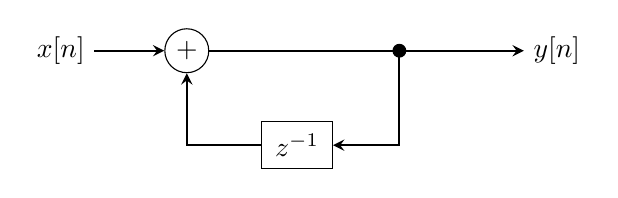
\begin{tikzpicture}[>=stealth]
    \node (x) at (0,0) {$x[n]$};
    \node[draw, circle, inner sep=2pt] (sum) at (1.6,0) {$+$};
    \coordinate (branch) at (4.3,0);
    \node (y) at (6.3,0) {$y[n]$};

    \node[
        draw,
        rectangle,
        minimum width=0.9cm,
        minimum height=0.6cm
    ] (delay) at (3,-1.2) {$z^{-1}$};

    \draw[->, thick] (x) -- (sum);
    \draw[thick] (sum) -- (branch);
    \fill (branch) circle (2.5pt);
    \draw[->, thick] (branch) -- (y);

    \draw[->, thick]
        (branch) |- (delay.east);

    \draw[->, thick]
        (delay.west) -| (sum.south);
\end{tikzpicture}
\end{center}
The impulse response is $h[n] = H\{\delta[n]\} = u[n]$. This system is
\textbf{not FIR}; it is \textbf{IIR} (Infinite Impulse Response).
\end{examplebox}

\noindent \textbf{Properties we will study:}
\HandoutSecLink{sec:linearity}{Linearity},
\HandoutSecLink{sec:time-invariance}{Time Invariance},
\HandoutSecLink{sec:causality}{Causality},
\HandoutSecLink{sec:impulse-response}{Impulse Response},
\HandoutSecLink{sec:convolution}{Convolution},
\HandoutSecLink{sec:stability}{Stability}.

\HandoutMarkSection{2}{Linear Discrete-Time Systems}\label{sec:linearity}

\begin{defbox}[title={Definition (Linearity)}]
For arbitrary $\alpha,\beta \in \C$ and arbitrary inputs $x_1[n]$ and
$x_2[n]$: if
\[
y_1[n] = H\{x_1[n]\}
\qquad
\left(x_1[n] \xrightarrow{H} y_1[n]\right)
\]
and if
\[
x_2[n] \xrightarrow{H} y_2[n],
\]
then if
\[
x[n] = \alpha x_1[n] + \beta x_2[n],
\]
we must have
\[
x[n] \xrightarrow{H} y[n]
= \alpha y_1[n] + \beta y_2[n].
\]
\end{defbox}

\begin{examplebox}[title={Example (Accumulator is Linear)}]
\[
y[n]=\sum_{\ell=-\infty}^{n}x[\ell]
\qquad
\text{(Accumulator)}
\]

\[
x_1[n] \xrightarrow{H} y_1[n]
= \sum_{\ell=-\infty}^{n} x_1[\ell]
\]

\[
x_2[n] \xrightarrow{H} y_2[n]
= \sum_{\ell=-\infty}^{n} x_2[\ell]
\]

If
\[
x[n]=\alpha x_1[n]+\beta x_2[n],
\]
then
\begin{align*}
x[n] \xrightarrow{H} y[n]
&= \sum_{\ell=-\infty}^{n}
   \left(\alpha x_1[\ell]+\beta x_2[\ell]\right) \\
&= \alpha\sum_{\ell=-\infty}^{n}x_1[\ell]
 + \beta\sum_{\ell=-\infty}^{n}x_2[\ell] \\
&= \alpha y_1[n]+\beta y_2[n].
\end{align*}

Therefore, the accumulator is linear.
\end{examplebox}

\HandoutMarkSection{3}{Homogeneity for the Accumulator,\\ via the Difference-Equation Form}

\begin{examplebox}[title={Example}]
\[
y[n] = y[n-1] + x[n]
\qquad
\text{(accumulator)}
\]

Assume
\[
x[n] \xrightarrow{H} y[n]
\]

Let
\[
x_1[n] = \alpha x[n] \xrightarrow{H} y_1[n]
\]

Then
\[
y_1[n] = y_1[n-1] + \alpha x[n], \qquad
\alpha y[n] = \alpha y[n-1] + \alpha x[n].
\]
Subtracting,
\begin{align*}
y_1[n] - \alpha y[n] &= y_1[n-1] - \alpha y[n-1] \\
&\Longrightarrow\ g[n] = g[n-1], \quad g[n] \triangleq y_1[n]-\alpha y[n].
\end{align*}
\end{examplebox}

\begin{notebox}
$g[n]$ should be zero for all $n$ for homogeneity to hold.

We assume
\textbf{zero initial conditions (ICs)} (a restrictive definition; we will
use something more general for LTI systems):
\begin{align*}
\exists\, M\in\Z \text{ s.t. } y[n]=0,\ x[n]=0,\ y_1[n]=0 \ \ \forall n\le M \\
\Longrightarrow\ g[n]=0\ \forall n\le M \\
\Longrightarrow\ g[n]=0\ \forall n.
\end{align*}
\noindent\HandoutMarkLeft{4}So $y_1[n] = \alpha y[n]$ for all $n$: \textbf{Homogeneity} $\checkmark$.
\end{notebox}

\begin{notebox}
Proving linearity is frequently harder than disproving linearity.
\end{notebox}

\begin{examplebox}[title={Example (Median Filter: Homogeneous but not Additive)}]
$y[n] = \median\{x[n-1], x[n], x[n+1]\}$.
\begin{itemize}
  \item Homogeneity? $\checkmark$
  \item Additivity? $\times$
\end{itemize}
For single impulses $x_1[n]$ and $x_2[n]$ at different locations, the median
filter outputs $y_1[n]$ and $y_2[n]$ that are each zero (or small); but for
$x_1[n]+x_2[n]$ (two nonzero samples), the median output $y[n] \ne
y_1[n]+y_2[n]$. Hence \textbf{additivity fails}.
\end{examplebox}

\HandoutMarkSection{5}{Time-Invariant Discrete-Time Systems}\label{sec:time-invariance}

\begin{defbox}[title={Definition (Time-Invariance)}]
For arbitrary $x[n]\xrightarrow{H}y[n]$: if $x_1[n] = x[n-n_0]$ for arbitrary
$n_0\in\Z$, then $x_1[n]\xrightarrow{H}y_1[n] = y[n-n_0]$.
\end{defbox}

\begin{examplebox}[title={Example (FIR Filter is Time-Invariant)}]
$$y[n] = \sum_{k=0}^{M-1}\alpha_k\,x[n-k] \quad \text{(FIR filter)}.$$
Let $x_1[n] = x[n-n_0]$. Then
$$y_1[n] = \sum_{k=0}^{M-1}\alpha_k\,x_1[n-k]
         = \sum_{k=0}^{M-1}\alpha_k\,x\big[(n-k)-n_0\big]
         \overset{?}{=} y[n-n_0] \ \Longrightarrow\ \textbf{time invariant!}$$
\end{examplebox}

\begin{examplebox}[title={Example (A System that is \emph{Not} Time-Invariant)}]
$$y[n] = \sum_{k=0}^{M-1}\alpha_k\,\symbfit{x}[n-k] + \symbfit{x}[0].$$
For $\symbfit{x}[n] = \delta[n]$:
$$y[n] = \begin{cases} \alpha_n + 1, & 0\le n\le M-1\\ 0+1, & \text{else}
\end{cases}.$$
\noindent\HandoutMarkLeft{6}For $\symbfit{x}_1[n] = \delta[n-1]$:
$$y_1[n] = \begin{cases} \alpha_{n-1} + 0, & 1\le n\le M\\ 0+0, & \text{else}
\end{cases}.$$
Since $y_1[n] \ne y[n-1]$ (the added constant $\symbfit{x}[0]$ does not shift),
\textbf{time invariant? Nope.}

\noindent The extra term always reads the input at index $0$, not at a lag
relative to $n$. Shifting the input by $n_0$ therefore does not translate
that contribution through time; the output is not a shifted copy of the
original response.
\end{examplebox}

\section{Linear Time-Invariant (LTI) Systems}

\begin{itemize}
  \item Linear
  \item Time-invariant
  \item Easy to analyze, characterize, implement, and design.
\end{itemize}

\subsection{Important Subclass: Linear Constant-Coefficient Difference Equations (LDEs)}

An important subclass, with zero ICs:
$$\sum_{k=0}^{N-1} d_k\,y[n-k] = \sum_{q=0}^{M-1} p_q\,x[n-q].$$
Solving for $y[n]$:
\begin{align*}
y[n] &= \sum_{k=1}^{N-1} \tilde d_k\,y[n-k] + \sum_{q=0}^{M-1}\tilde p_q\,x[n-q], \\
&\quad\left(\tilde d_k = -\frac{d_k}{d_0}, \quad \tilde p_q = \frac{p_q}{d_0};\ \text{assuming } d_0 \ne 0\right).
\end{align*}

\begin{examplebox}[title={Examples: Accumulator (FIR Filter)}, handout mark=7]
$$y[n] = y[n-1] - x[n-1] + \rho\big(y[n-1]-x[n-1]\big),$$
where $y[n]$ is the loan balance, $y[n-1]$ the previous balance, $x[n-1]$
the payment, and $\rho$ the interest rate.
Similar in spirit to the continuous-time ODE form
$$y(t) = \sum_{n=0}^{N} \alpha_n\frac{d^n x(t)}{dt^n}
  + \sum_{m=1}^{M} \beta_m\frac{d^m y(t)}{dt^m}.$$
\end{examplebox}

\section{Causal Systems}\label{sec:causality}

\begin{defbox}[title={Definition (Causality)}]
The $m$th output sample $y[m]$ depends only on input samples $x[n]$ with
$n \le m$. This must be true for all possible inputs and all $m$.
\end{defbox}

\begin{examplebox}[title={Examples}]
\begin{itemize}
  \item $y[n] = \median\{x[n-1],x[n],x[n+1]\}$: \textbf{not causal}.
  \item $y[n] = y[n-1] + x[n]$: causal, with an IC.
  \item $y[n] = \sum_{k=0}^{M-1}\alpha_k\,x[n-k]$: \textbf{causal}.
  \item $y[n] = \sum_{k=0}^{M-1}\alpha_k\,x[n-k] + x[0]$: \textbf{not causal}.
\end{itemize}
\end{examplebox}

\begin{factbox}[title={Property (Causal Systems and Matching Inputs)}, handout mark=8]
For a causal system, if $x_1[n]\xrightarrow{H}y_1[n]$ and
$x_2[n]\xrightarrow{H}y_2[n]$, and if $x_1[n]=x_2[n]$ for all $n<N$, and the
ICs are the same, then $y_1[n] = y_2[n]$ for all $n<N$.
\end{factbox}

\section{Stability}\label{sec:stability}

\begin{defbox}[title={Definition (BIBO Stability)}]
A system is \textbf{bounded-input bounded-output (BIBO) stable} if every
bounded input yields a bounded output, i.e., if $|x[n]| \le B_x < \infty$
for all $n$, then $|y[n]| \le B_y < \infty$ for all $n$.
\end{defbox}

\begin{examplebox}[title={Example (Moving Average is BIBO Stable)}, handout mark=9]
\[
y[n] = \frac{1}{M}\sum_{k=0}^{M-1}x[n-k].
\]

Assume
\[
|x[n]| \le B_x < \infty \quad \text{for all } n.
\]

Then
\begin{align*}
|y[n]|
&= \left|\frac{1}{M}\sum_{k=0}^{M-1}x[n-k]\right| \\
&\le \frac{1}{M}\sum_{k=0}^{M-1}|x[n-k]| \\
&\le \frac{1}{M}\sum_{k=0}^{M-1}B_x = B_x
\ \Longrightarrow\ \textbf{BIBO stable!}
\end{align*}
\end{examplebox}

\begin{examplebox}[title={Example (Accumulator is \emph{Not} BIBO Stable)}]
$y[n] = y[n-1] + x[n]$, with IC $y[n]=x[n]=0$ for $n<0$. Let $x[n]=u[n]$
(bounded). Then $y[n] = (n+1)u[n]$, which is \textbf{not bounded}.
\end{examplebox}

\section{Impulse Response}\label{sec:impulse-response}

\begin{defbox}[title={Definition (Impulse Response)}]
The impulse response $h[n]$ is the output of a discrete-time system to the
input $\delta[n]$.
\end{defbox}

\begin{examplebox}[title={Example (Accumulator)}]
$$y[n] = \sum_{k=-\infty}^{n} x[k] \ \Longrightarrow\
  h[n] = \sum_{k=-\infty}^{n}\delta[k] = u[n].$$
\end{examplebox}

\begin{factbox}[title={Fact}, handout mark=10]\label{sec:convolution}
LTI systems with zero ICs are \textbf{completely characterized} by their
impulse responses.
\end{factbox}

\begin{notebox}
A more general definition of zero ICs for LTI systems: if $x[n]=0$ for all
$n$, then $y[n] = H\{x[n]\} = 0$ for all $n$: ``zero-input'' $\Rightarrow$
``zero-output.'' (Non-zero ICs $\Rightarrow$ not LTI.)

\emph{Proof of fact:} next time.
\end{notebox}

\section*{Readings}
\begin{itemize}
  \item Sanjit K. Mitra, \textit{Digital Signal Processing: A Computer-Based Approach}, 4th ed., Ch.\ 4.5--4.7
  \item Monson H. Hayes, \textit{Schaum's Outline of Digital Signal Processing}, 2nd ed., Ch.\ 1.5, 2.4
\end{itemize}

\HandoutAppendixListStart
  \HandoutAppendixListItem{app:mitra}{A.\ Sanjit K. Mitra, \textit{Digital Signal Processing: A Computer-Based Approach}, 4th ed., Ch.\ 4.5--4.7}
  \HandoutAppendixListItem{app:scan}{B.\ Handwritten Lecture Note Scan (September 1, 2026)}
\HandoutAppendixListEnd

\HandoutAppendixSection{app:mitra}{Mitra, Ch.\ 4.5--4.7}
\HandoutIncludeTextbookExcerpt{Mitra-4.5-4.7.pdf}

\HandoutAppendixSection{app:scan}{Handwritten Lecture Note Scan}
\HandoutIncludeHandoutScan{lecture3_0901.pdf}

\end{document}
